\documentclass[11pt]{article}

% =============================================================================
%  style.tex — the paper's design system.
%
%  Single-column modern-preprint layout: XCharter for text, Fira Sans for
%  headings and captions, Inconsolata for code. Colours are the same three
%  categorical slots the figures use (paper/figures/style.py), so a reader
%  never has to relearn what blue and orange mean between a figure and the
%  prose around it.
% =============================================================================

% ---------------------------------------------------------------- geometry --
\usepackage[
  letterpaper,
  top=1.05in, bottom=1.05in, left=1.10in, right=1.10in,
  footskip=0.45in, headsep=0.22in
]{geometry}

% ------------------------------------------------------------------- fonts --
\usepackage[T1]{fontenc}
\usepackage{XCharter}
\usepackage[scaled=0.93]{FiraSans}
\usepackage[varqu,varl,scaled=0.92]{inconsolata}
\usepackage[charter,vvarbb,scaled=1.04]{newtxmath}
\usepackage{microtype}

\linespread{1.045}
\setlength{\emergencystretch}{1.6em}   % long \texttt{} runs must not overflow

% ------------------------------------------------------------------ colours --
\usepackage[table,dvipsnames]{xcolor}

\definecolor{arblue}{HTML}{2A78D6}    % autoregressive  (categorical slot 1)
\definecolor{dgorange}{HTML}{EB6834}  % block diffusion (categorical slot 2)
\definecolor{llaqua}{HTML}{1BAF7A}    % LLaDA           (categorical slot 3)

\definecolor{ink}{HTML}{0B0B0B}
\definecolor{ink2}{HTML}{52514E}
\definecolor{muted}{HTML}{898781}
\definecolor{rule}{HTML}{C3C2B7}
\definecolor{hairline}{HTML}{E8E7E1}

\definecolor{washblue}{HTML}{EAF1FB}
\definecolor{washorange}{HTML}{FDEEE7}
\definecolor{washneutral}{HTML}{F4F3F0}

\definecolor{deepink}{HTML}{1B3A5C}    % heading ink — a calm dark blue

% ------------------------------------------------------------------ tables --
\usepackage{booktabs}
\usepackage{array}
\usepackage{multirow}
\usepackage{tabularx}
\renewcommand{\arraystretch}{1.18}
\setlength{\tabcolsep}{6pt}
\newcolumntype{R}{>{\raggedleft\arraybackslash}X}
\newcolumntype{L}{>{\raggedright\arraybackslash}X}

% Table body in the sans face at a slightly smaller size — numbers read
% better and the table separates cleanly from the surrounding text.
\newcommand{\tabfont}{\sffamily\footnotesize}
\newcommand{\thead}[1]{\textcolor{ink2}{\footnotesize\textbf{#1}}}

% --------------------------------------------------------------- headings ---
\usepackage{titlesec}

\titleformat{\section}
  {\normalfont\sffamily\large\bfseries\color{deepink}}
  {\textcolor{arblue}{\thesection}}{0.7em}{}
\titlespacing*{\section}{0pt}{1.55\baselineskip}{0.55\baselineskip}

\titleformat{\subsection}
  {\normalfont\sffamily\normalsize\bfseries\color{deepink}}
  {\textcolor{muted}{\thesubsection}}{0.6em}{}
\titlespacing*{\subsection}{0pt}{1.15\baselineskip}{0.35\baselineskip}

\titleformat{\subsubsection}
  {\normalfont\sffamily\small\bfseries\color{ink2}}
  {}{0em}{}
\titlespacing*{\subsubsection}{0pt}{0.9\baselineskip}{0.25\baselineskip}

\titleformat{\paragraph}[runin]
  {\normalfont\sffamily\small\bfseries\color{ink}}
  {}{0em}{}[.]
\titlespacing*{\paragraph}{0pt}{0.7\baselineskip}{0.55em}

% --------------------------------------------------------------- captions ---
\usepackage[font=small,labelfont={sf,bf,color=deepink},
            textfont={color=ink2},labelsep=period,
            skip=7pt,justification=justified]{caption}
\usepackage{subcaption}

% ------------------------------------------------------------------- boxes --
\usepackage[most]{tcolorbox}

% A key-result callout: tinted panel, coloured left rule, sans heading.
\newtcolorbox{keybox}[1][]{
  enhanced, breakable,
  colback=washneutral, colframe=washneutral,
  boxrule=0pt, leftrule=2.2pt,
  borderline west={2.2pt}{0pt}{arblue},
  arc=0pt, outer arc=0pt,
  left=9pt, right=9pt, top=7pt, bottom=7pt,
  before skip=9pt, after skip=9pt,
  fontupper=\small,
  #1
}

% A "what this section establishes" strip, used once per major section.
\newtcolorbox{takeaway}[1][]{
  enhanced, breakable,
  colback=washblue!55!white, colframe=washblue!55!white,
  boxrule=0pt, arc=1.5pt, outer arc=1.5pt,
  left=9pt, right=9pt, top=6pt, bottom=6pt,
  before skip=9pt, after skip=9pt,
  fontupper=\small,
  #1
}

% A caution/limitation strip — for scope conditions the reader must carry.
\newtcolorbox{caution}[1][]{
  enhanced, breakable,
  colback=washorange!60!white, colframe=washorange!60!white,
  boxrule=0pt, leftrule=2.2pt,
  borderline west={2.2pt}{0pt}{dgorange},
  arc=0pt, outer arc=0pt,
  left=9pt, right=9pt, top=6pt, bottom=6pt,
  before skip=9pt, after skip=9pt,
  fontupper=\small,
  #1
}

\newcommand{\boxhead}[1]{%
  \textcolor{deepink}{\sffamily\bfseries\footnotesize\MakeUppercase{#1}}\par
  \vspace{2pt}}

% ------------------------------------------------------------------- lists --
\usepackage{enumitem}
\setlist[itemize]{leftmargin=1.15em,itemsep=2.5pt,topsep=4pt,parsep=0pt}
\setlist[enumerate]{leftmargin=1.5em,itemsep=2.5pt,topsep=4pt,parsep=0pt}

% -------------------------------------------------------------------- misc --
\usepackage{amsmath}
\let\Bbbk\relax          % newtxmath already defines it
\usepackage{amssymb}
\usepackage{siunitx}
\sisetup{group-separator={,},group-minimum-digits=4,detect-all}
\usepackage{graphicx}
\usepackage{algorithm}
\usepackage{algpseudocode}
\usepackage{float}
\usepackage[hidelinks]{hyperref}
\hypersetup{
  colorlinks=true,
  linkcolor=arblue, citecolor=arblue, urlcolor=arblue,
  pdfborder={0 0 0}
}

% Model shorthands — one spelling per model, everywhere.
\newcommand{\ARthree}{\textsc{ar-3b}}
\newcommand{\ARoneb}{\textsc{ar-1.5b}}
\newcommand{\DG}{\textsc{dg}}
\newcommand{\LLaDA}{\textsc{llada-8b}}

% Coloured inline model tags, matching the figures.
\newcommand{\artag}{\textcolor{arblue}{\sffamily\bfseries AR}}
\newcommand{\dgtag}{\textcolor{dgorange}{\sffamily\bfseries DG}}

% A quiet inline source pointer.
\newcommand{\artifact}[1]{\textcolor{muted}{\ttfamily\scriptsize #1}}

% ---------------------------------------------------------------- title page --
\usepackage{titling}
\usepackage{fancyhdr}

\pagestyle{fancy}
\fancyhf{}
\renewcommand{\headrulewidth}{0pt}
\fancyfoot[C]{\textcolor{muted}{\sffamily\footnotesize\thepage}}

% \papertitle{title}{subtitle}{author}{affiliation}{version line}
\newcommand{\papertitle}[5]{%
  \thispagestyle{empty}
  \begingroup
  \raggedright\parindent=0pt
  {\sffamily\bfseries\fontsize{21}{25}\selectfont\color{deepink} #1\par}
  \vspace{5pt}
  {\sffamily\fontsize{13}{16}\selectfont\color{ink2} #2\par}
  \vspace{8pt}
  {\color{arblue}\rule{\linewidth}{2pt}\par}
  \vspace{9pt}
  {\sffamily\large\color{ink} #3\par}
  \vspace{2pt}
  {\sffamily\small\color{ink2} #4\par}
  \vspace{3pt}
  {\sffamily\footnotesize\color{muted} #5\par}
  \endgroup
  \vspace{16pt}
}

% =============================================================================
%  macros.tex — every number the paper cites, in one place.
%
%  Rule: no numeral is typed into a section file. If it is a measurement, it
%  is a macro here, and the comment on its line names the artifact it was read
%  from. paper/verify_numbers.py re-reads those artifacts; the figure builder
%  (paper/figures/make_figures.py) prints what it plotted so the two can be
%  diffed.
% =============================================================================

% --- Pinned stack -------------------------------------------------- (#57) --
\newcommand{\vllmVersion}{0.25.1}
\newcommand{\torchVersion}{2.11.0+cu130}
\newcommand{\gpuModel}{NVIDIA A100 80GB PCIe}
\newcommand{\nPerCell}{300}
\newcommand{\refPrompt}{1{,}047}

% --- Quality, 9-field vs 12-field ----- results/issue43_nine_field_f1.json --
\newcommand{\arThreeBFnine}{0.8516}     % AR-3B,  L=256, 9-field
\newcommand{\dgNineF}{0.8518}           % DG,     L=256, 9-field
\newcommand{\arThreeBFtwelve}{0.8263}   % AR-3B,  L=256, 12-field
\newcommand{\dgTwelveF}{0.7858}         % DG,     L=256, 12-field
\newcommand{\qualityGap}{0.0002}        % |9-field difference|
\newcommand{\twelveGap}{0.0405}         % 12-field difference, AR-favoured
% AR-1.5B: results/issue_evidence_ar1b_{L512,L1024,energy}.json (pinned stack)
\newcommand{\arOneFiveFnine}{0.8679}

% --- Cost laws ------------- results/anchors/*.json, results/issue68_*.json --
\newcommand{\arBase}{7.27}        % ms, AR fitted intercept
\newcommand{\arSlope}{6.29}       % ms/token, AR fitted decode slope
\newcommand{\dgBase}{378.8}       % ms, DG base at K=8
\newcommand{\dgStep}{119.5}       % ms, median of the 7 measured canvas steps
\newcommand{\dgStepLo}{113.1}     % ms, smallest measured step (1536->1792 in)
\newcommand{\dgStepHi}{122.6}     % ms, largest measured step (256->512)
\newcommand{\canvasLength}{256}   % tokens per canvas
\newcommand{\dgMarginal}{0.47}    % ms/token at the margin: step / canvas
\newcommand{\marginalRatio}{13.5} % arSlope / dgMarginal

% Anchors, five repeats each -------- results/anchors/anchor_remeasure.json --
\newcommand{\arAnchorTwoFive}{1616.0}   % AR-3B  L=256 p50, CV 0.05%
\newcommand{\arAnchorFiveOne}{3225.1}   % AR-3B  L=512 p50, CV 0.01%
\newcommand{\dgAnchorTwoFive}{379.0}    % DG     L=256 p50, CV 0.25%
\newcommand{\dgAnchorFiveOne}{500.7}    % DG     L=512 p50, CV 0.12%
\newcommand{\arCV}{0.05}
\newcommand{\dgCV}{0.25}
% Per-event dispersion within one run -- results/anchors/*_L256_r1_preds.jsonl
\newcommand{\arEventCV}{0.17}     % % CV over 300 per-event latencies
\newcommand{\dgEventCV}{20.9}
\newcommand{\arMaxMed}{1.03}      % max / median per-event latency
\newcommand{\dgMaxMed}{3.21}

% --- Crossovers ------------------------- models/decision/procedure.py --------
\newcommand{\crossoverL}{59}       % tokens: (dgBase - arBase) / arSlope
\newcommand{\crossoverLambda}{2.6} % ev/s:   1000 / dgBase
\newcommand{\naturalLdg}{176}      % DG natural output length (tokens)
\newcommand{\naturalLar}{123}      % AR natural output length (tokens)

% --- Input length, the second variable ------ results/issue44_*_sweep.json --
\newcommand{\arInputSlope}{0.047}  % ms per prompt token
\newcommand{\dgInputSlope}{0.123}  % ms per prompt token
\newcommand{\inputSlopeRatio}{2.6} % dgInputSlope / arInputSlope

% --- Base decomposition ------------------- results/issue44_dg_ksweep_K*.json --
\newcommand{\kfitBase}{296.1}      % ms, K-independent term
\newcommand{\kfitSlope}{2.57}      % ms per denoising step
\newcommand{\kfitRsq}{0.49}
\newcommand{\dgPrefillPct}{93.5}   % share of the fitted cost that is prefill
\newcommand{\dgDenoisePct}{6.5}    % share that is the denoising loop

% --- Batching ------------------- results/issue42_batching.json, appD, dInfer --
\newcommand{\arBatchMult}{80}      % typical AR multiplier (77-86x range)
\newcommand{\arBatchLo}{77.1}      % vLLM, L=128
\newcommand{\arBatchHi}{86.0}      % vLLM, L=512
\newcommand{\cacheOnMult}{42.8}    % AR-3B, prefix caching on   (#42)
\newcommand{\cacheOffMult}{26.8}   % AR-3B, prefix caching off  (#42)
\newcommand{\dgBatchMult}{1.18}    % LLaDA-8B under dInfer, flat to batch 64
\newcommand{\dgBatchVllmLo}{1.5}   % DG under vLLM, L=512 (lower bound)
\newcommand{\dgBatchVllmHi}{1.7}   % DG under vLLM, L=128 (lower bound)

% --- Energy -------------------------- results/issue_energy_measurement.json --
\newcommand{\arThreeEnergy}{22.3}  % J/event, net of idle, forced L=256
\newcommand{\dgEnergy}{4.2}        % J/event, net of idle, forced L=256
\newcommand{\arOneFiveEnergy}{5.1} % J/event, net of idle, forced L=256
\newcommand{\energyRatio}{4.3}     % arThreeEnergy / dgEnergy

% --- Deployment pair ------ results/issue_evidence_ar1b_*.json, issue68_*.json --
\newcommand{\arOneFiveTwoFive}{1007}   % ms, AR-1.5B forced L=256
\newcommand{\arOneFiveFiveOne}{2005}   % ms, AR-1.5B forced L=512
\newcommand{\arOneFiveTenTwoFour}{4026}% ms, AR-1.5B forced L=1024
\newcommand{\dgTwoFive}{378}           % ms, DG forced L=256
\newcommand{\dgFiveOne}{501}           % ms, DG forced L=512
\newcommand{\dgTenTwoFour}{739}        % ms, DG forced L=1024
\newcommand{\arOneFiveWeights}{3.0}    % GB, bf16
\newcommand{\dgWeights}{52.0}          % GB, bf16
\newcommand{\footprintRatio}{17}       % dgWeights / arOneFiveWeights

% --- Defect magnitudes ------------------------------ CHECKLIST.md, #65 -----
\newcommand{\defectOneFBefore}{0.779}
\newcommand{\defectOneFAfter}{0.844}
\newcommand{\defectTwoBefore}{1841.6}
\newcommand{\defectTwoAfter}{413.3}
\newcommand{\defectTwoRatio}{4.5}
\newcommand{\defectThreeBefore}{0.599}
\newcommand{\defectThreeAfter}{0.826}
\newcommand{\defectFourBefore}{0}
\newcommand{\defectFourAfter}{100}
\newcommand{\rambleRate}{96}      % % of AR outputs with >1 JSON object at L=512

% --- Truncation regime -------------------------- results/issue43/*.json -----
\newcommand{\arFOneTwentyEight}{0.669}   % AR-3B 9-field F1 at L=128
\newcommand{\dgFOneTwentyEight}{0.311}   % DG    9-field F1 at L=128
\newcommand{\arValidTwentyEight}{66.7}   % AR schema-valid % at L=128
\newcommand{\dgValidTwentyEight}{1.0}    % DG schema-valid % at L=128

% --- Generalisation to HDFS ---------------------- results/issue67_*.json ----
\newcommand{\hdfsStep}{120.5}     % ms, DG canvas step on HDFS
\newcommand{\bglStep}{118.5}      % ms, DG canvas step on BGL (same cells)
\newcommand{\arHdfs}{1616.5}      % ms, AR-3B L=256 on HDFS
\newcommand{\arBgl}{1616.0}       % ms, AR-3B L=256 on BGL

% --- Canvas tuning -------------------------- results/issue66_canvas_*.json --
\newcommand{\canvasOneTwentyEightBase}{368.5}  % ms at canvas=128
\newcommand{\canvasOneTwentyEightFone}{0.8644} % 9-field F1 at canvas=128

% --- K as a runtime quality knob --------- results/issue44_dg_ksweep_K*.json --
\newcommand{\kFourPfifty}{292}    % ms
\newcommand{\kFourPninetynine}{394.3} % ms
\newcommand{\kFourFone}{0.790}
\newcommand{\kEightPfifty}{379}   % ms
\newcommand{\kEightFone}{0.853}
\newcommand{\kTwoPfifty}{202}     % ms
\newcommand{\kTwoFone}{0.485}

% --- Superseded values, cited only when discussing the discrepancy ----------
\newcommand{\dgOldBase}{418.2}    % ms, DG base at K=32
\newcommand{\arOldPfifty}{1617.6} % ms, AR-3B L=256, Campaign B

\graphicspath{{../}}

\begin{document}

\papertitle
  {The Cost Shape of Block-Structured Decoding}
  {When diffusion LLMs win, and why they usually don't}
  {Aleksandr Kaigorodov}
  {Yandex}
  {Preprint \textperiodcentered\ August 2026 \textperiodcentered\ v0}

% ---------------------------------------------------------------- abstract --
\begingroup
\small
\noindent
{\sffamily\bfseries\footnotesize\color{deepink}ABSTRACT}\par
\vspace{3pt}
\noindent
Autoregressive and block-diffusion language models reach the same quality on
structured log extraction --- 9-field macro F1 differs by \qualityGap\ at the
compute-matched pair --- but their inference costs have different
\emph{shapes}. Autoregressive cost is a line in output length with no floor:
\arBase~ms plus \arSlope~ms per token. Block-diffusion cost is a staircase
with a prefill-dominated floor: \dgBase~ms for the first canvas of
\canvasLength\ tokens, then \dgStep~ms for each additional canvas. We measure
both laws on one pinned serving stack with run-to-run coefficient of variation
below $0.3\%$, verify that the staircase has sharp edges exactly at canvas
boundaries, and show that the shapes generalise from BGL to HDFS within
$1.7\%$. The shapes cross at $L^{*} \approx \crossoverL$ output tokens, below
which the autoregressive model is cheaper per event. We turn the two laws into
an executable decision procedure over (output length, arrival rate, batching
availability, quality tolerance), and then ask whether the crossover survives
a fair deployment comparison. It does not, at short output: the
quality-matched autoregressive model is \footprintRatio$\times$ smaller,
converts arrival concurrency into throughput at \arBatchMult$\times$ against
the diffusion model's \dgBatchMult$\times$, and pays \inputSlopeRatio$\times$
less per prompt token. What survives is narrower and real --- at forced output
$L \geq 512$ under a batch-1 constraint, the diffusion model is
$4.0$--$5.4\times$ faster than the quality-matched baseline, uses less energy,
and degrades under deadline pressure by losing quality rather than
completeness. We also report five defects in our own measurement harness, four
of which biased against the autoregressive baseline, each found by re-reading
committed artifacts rather than by running new experiments.
\endgroup

\vspace{4pt}

% ----------------------------------------------------- findings at a glance --
\begin{keybox}
\boxhead{The paper in one table}
\vspace{-2pt}
\begin{tabularx}{\linewidth}{@{}L r r@{}}
\toprule
\tabfont & \thead{\ARthree} & \thead{\DG-26B-A4B} \\
\midrule
\tabfont 9-field macro F1 ($L{=}\canvasLength$)      & \arThreeBFnine & \dgNineF \\
\tabfont Active parameters                            & 3.0\,B & 4.0\,B \\
\tabfont p50 latency at $L{=}\canvasLength$, batch-1  & \arAnchorTwoFive\,ms & \dgAnchorTwoFive\,ms \\
\tabfont Marginal cost per output token               & \arSlope\,ms & \dgMarginal\,ms \\
\tabfont Marginal cost per prompt token               & \arInputSlope\,ms & \dgInputSlope\,ms \\
\tabfont Batch-1 $\to$ peak throughput multiplier     & \arBatchLo--\arBatchHi$\times$ & \dgBatchMult$\times$ \\
\tabfont Energy per event, net of idle                & \arThreeEnergy\,J & \dgEnergy\,J \\
\bottomrule
\end{tabularx}
\vspace{3pt}
\par\footnotesize\textcolor{ink2}{%
The diffusion model wins the first column of a latency table and loses the
deployment comparison behind it. \S\ref{sec:fair} works out why, and
\S\ref{sec:decision} makes the trade executable.}
\end{keybox}

\vspace{2pt}

\section{Introduction}
\label{sec:intro}

An autoregressive language model pays one forward pass per output token, so
its latency is a line: double the record you ask it to emit and you double the
wait. A block-diffusion language model does something structurally different.
It writes onto a fixed-size \emph{canvas} --- \canvasLength\ tokens, in the
model we measure --- and denoises every position on that canvas in parallel,
in a fixed number $K$ of steps. Inside a canvas, emitting one token and
emitting \canvasLength\ of them cost the same. The cost only moves when the
output crosses a canvas boundary, and then it moves in a step.

These are two different \emph{shapes}, not two points on one scale, and the
difference is the subject of this paper. A line with no floor and a staircase
with a high one will cross exactly once in the first canvas, and everything a
deployment cares about --- which model is cheaper, at what output length, at
what arrival rate, at what memory budget --- follows from where that crossing
sits relative to the workload. Figure~\ref{fig:cost-shapes} is the whole
argument in one picture.

\begin{figure}[t]
\centering
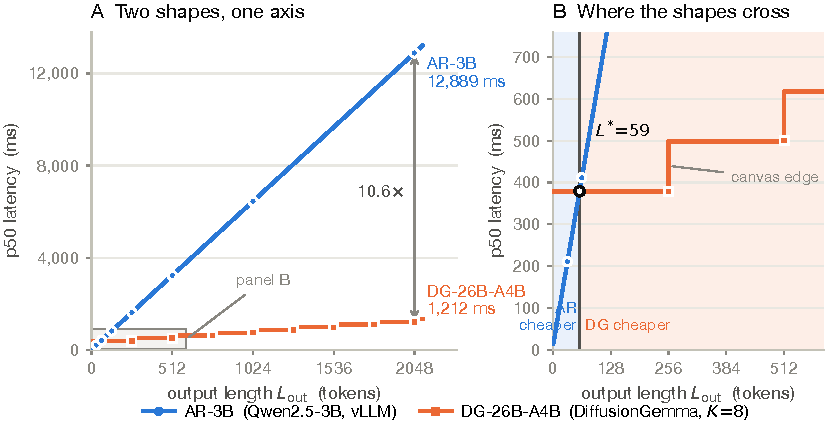
\includegraphics[width=\linewidth]{figures/fig1_cost_shapes.pdf}
\caption{The two cost shapes, measured on one pinned stack (vLLM
\vllmVersion, \gpuModel, BF16, batch-1). Markers are measured p50 latencies;
lines are the fitted laws. \textbf{A:} across the full sweep the
autoregressive model reaches \num{12889}\,ms at $L{=}2048$ while the diffusion
model reaches \num{1212}\,ms --- but the two curves are not the same kind of
object. \textbf{B:} inside the first canvas the diffusion cost is flat at its
floor, so the shapes cross once, at $L^{*}\approx\crossoverL$ tokens. Beyond
the crossover the diffusion model is cheaper, and each canvas edge widens the
gap by \dgStep\,ms against the autoregressive model's
$\arSlope\times\canvasLength \approx \num{1610}$\,ms.}
\label{fig:cost-shapes}
\end{figure}

\paragraph{Why this is worth measuring carefully}
Diffusion language models are routinely advertised as a low-latency route to
structured generation, and the argument is architecturally sound as far as it
goes. But reported speedups are almost always measured against an
autoregressive baseline built by the same authors, and constructing that
baseline is not a neutral act. The decoding configuration, the serving
runtime, the parser, and the metric are each worth a multiple. This project
began as an attempt to reproduce one such claim and found, instead, five
defects in \emph{its own} harness --- four of them biasing against the
autoregressive arm, each large enough to move a headline number by more than
the effect being reported (\S\ref{sec:setup}). We report them first, because
every number after them depends on their being fixed.

\paragraph{What we measure, and on what}
One task: extracting a 12-field structured record from a raw log line, scored
on the nine fields that carry discriminative signal (\S\ref{sec:exchange}).
Two corpora: BGL and HDFS from LOGHUB. One serving stack, pinned from issue
\#57 onward: vLLM \vllmVersion\ on an \gpuModel. Two models at the
compute-matched pair --- Qwen2.5-3B~\cite{qwen25} (\ARthree, 3.0\,B dense, all
active) against DiffusionGemma-26B-A4B~\cite{diffusiongemma} (\DG, 26\,B
total, 4.0\,B active through a top-8-of-128 mixture of experts) --- plus
Qwen2.5-1.5B as the \emph{quality}-matched baseline, and
LLaDA-8B~\cite{llada2025} on a second, diffusion-native runtime as a control. Run-to-run coefficient of variation on the pinned stack
is \arCV\% for the autoregressive arm and \dgCV\% for the diffusion arm over
five repeats of $n{=}\nPerCell$ events, so the effects below are not noise.

\paragraph{Contributions}
\begin{itemize}
  \item \textbf{Two fitted cost laws, and the mechanism behind the shapes.}
    $T_{\textsc{ar}} = \arBase + \arSlope\,L_{\mathrm{out}}$;
    $T_{\textsc{dg}} = \dgBase + \dgStep\,(\lceil
    L_{\mathrm{out}}/\canvasLength\rceil - 1)$. We show the staircase has
    sharp edges at exactly the canvas boundary (crossing one costs
    $\sim$120\,ms; staying inside costs under 1\,ms), that all seven measured
    steps are the same step, and that the shape survives a change of corpus.
    We also decompose the diffusion base and find that the denoising loop ---
    the part that makes the model ``diffusion'' --- is only \dgDenoisePct\% of
    it. The shape comes from the \emph{block}, not from the diffusion
    (\S\ref{sec:laws}).
  \item \textbf{A second variable, stated as a scope condition rather than
    buried.} Diffusion cost also depends on \emph{input} length, at
    \dgInputSlope\,ms per prompt token against the autoregressive model's
    \arInputSlope{} --- \inputSlopeRatio$\times$ steeper, because each denoising
    step re-attends the whole prompt. Every one-variable claim in this paper is
    calibrated at a \refPrompt-token prompt and must not be extrapolated past
    it.
  \item \textbf{An executable decision procedure.} Four inputs, five guards,
    every constant traced to a committed artifact, 11/11 self-tests passing,
    runnable from a clean checkout with no GPU (\S\ref{sec:decision}).
  \item \textbf{A fair comparison that closes the crossover, and the niche
    that survives it.} At the quality-matched pair the autoregressive model is
    \footprintRatio$\times$ smaller, batches \arBatchMult$\times$ better, and
    pays less per prompt token; the per-event advantage does not survive any
    of the three. What does survive is forced long output under a batch-1
    constraint, where the diffusion model is $4.0$--$5.4\times$ faster, uses
    less energy, and --- unlike the autoregressive model --- degrades under a
    deadline by losing quality rather than completeness (\S\ref{sec:fair}).
  \item \textbf{Negative results at the same length as the positive ones.} Six
    hypotheses of ours were refuted and three earlier claims withdrawn,
    including a prediction that diffusion would be more robust to input
    perturbation, which failed in 10 of 10 categories
    (\S\ref{sec:negative}).
\end{itemize}

\paragraph{What this paper is not}
It is not a claim that diffusion decoding is slow. It is a claim about where a
particular cost \emph{shape} puts a particular model in a particular
deployment plane, measured on one GPU, one runtime, one task family, and two
corpora. \S\ref{sec:threats} states the limits before a reviewer has to, and
the largest of them --- that our two arms are matched on active compute rather
than on size --- is the reason \S\ref{sec:fair} exists at all.

\section{Setup, and What We Got Wrong First}
\label{sec:setup}

This section is partly a methods description and partly an audit. The audit
comes first, because five defects in our own comparison harness biased the
measurements before any architectural conclusion could be drawn, and four of
the five biased the same way --- against the autoregressive baseline. We found
all five by re-reading committed artifacts, not by running new experiments,
and the corrections moved headline numbers by more than the effects we had
been reporting. That makes them a result, not a footnote.

\subsection{The stack everything is measured on}

Every measurement from issue \#57 onward runs on a single pinned stack
(Table~\ref{tab:stack}). A shared provenance helper, which no runner can
bypass, writes the model id, revision, runtime versions, GPU, dtype, and every
decoding knob into each result file --- taken from the object that actually
loaded the model, not from a command-line default. A build check
(\artifact{paper/verify\_numbers.py}) fails when a cited artifact lacks that
block. The helper exists because it had to: three result files recorded an
autoregressive model name for diffusion runs (defect 5, below).

\begin{table}[h]
\centering
\caption{The pinned stack. Every number in this paper is measured here unless
explicitly labelled otherwise.}
\label{tab:stack}
\begin{tabular}{@{}ll@{}}
\toprule
\thead{Component} & \thead{Version} \\
\midrule
\tabfont Serving runtime & \tabfont vLLM \vllmVersion~\cite{vllm2023} \\
\tabfont Framework       & \tabfont torch \torchVersion \\
\tabfont Accelerator     & \tabfont \gpuModel \\
\tabfont Precision       & \tabfont BF16 \\
\tabfont Diffusion scheduling & \tabfont serial, \texttt{-{}-max-num-seqs 1} \\
\tabfont Sample size     & \tabfont $n = \nPerCell$ events per cell \\
\bottomrule
\end{tabular}
\end{table}

The serial-diffusion setting is forced, not chosen: vLLM \vllmVersion\ crashes
in \artifact{diffusion\_gemma.py} as soon as two running requests mix
denoising phases. Serialised serving is therefore the diffusion arm's
production-relevant mode on this runtime, and \S\ref{sec:batching} treats that
as the finding it is rather than as an inconvenience.

\subsection{Task and metric}

The task is log-to-record extraction: given one raw log line from
LOGHUB~\cite{loghub} (BGL for the main sweeps, HDFS for the generalisation
check), emit a JSON record. The prompt is a few-shot template of roughly \refPrompt\ tokens.
Quality is macro F1 over fields, and we score \emph{nine} of the twelve
schema fields. The three we drop --- \texttt{event\_type},
\texttt{affected\_entity}, \texttt{remediation\_hint} --- have degenerate gold
labels on BGL: across 2{,}000 events they take 2, 1, and 1 unique values
respectively, so a model that emits an empty object scores $1.000$ on two of
the three by trivially matching a constant. \S\ref{sec:exchange} shows what
that contamination does to the comparison. Both metrics are computed on every
run; only the 9-field number is cited in comparison tables.

\subsection{Five defects, four of them one-sided}

\begin{figure}[t]
\centering
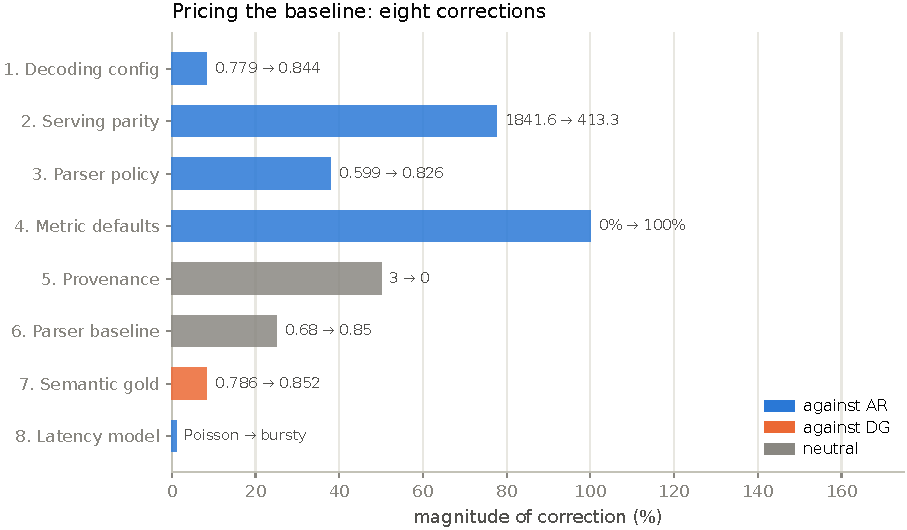
\includegraphics[width=\linewidth]{figures/fig8_defects.pdf}
\caption{Five defects in our own harness. Each row is one defect: the value
as originally recorded, the value after the fix, and which arm the bias
favoured. The four autoregressive-biased defects live in the
\emph{infrastructure the model runs on} --- its checkpoint defaults, its
serving path, its over-generation behaviour, its early-stopping behaviour ---
not in the model itself.}
\label{fig:defects}
\end{figure}

\paragraph{1. Decoding configuration}
HuggingFace \texttt{generate()} honours \texttt{repetition\_penalty} even
under \texttt{do\_sample=False}, and Qwen2.5 ships a checkpoint default of
1.1 at 1.5\,B and 1.05 at 3\,B/7\,B. Extraction consists almost entirely of
copying spans out of the input, which is exactly what that penalty suppresses:
it emptied the \texttt{host} field on 80 of 100 events. DiffusionGemma's
hand-written denoising loop has no equivalent default, so the handicap was
one-sided. Setting every knob explicitly on both arms moved \ARoneb\ Field-F1
from \defectOneFBefore\ to \defectOneFAfter.

\paragraph{2. Serving parity}
The autoregressive arm ran a naive HuggingFace generation loop while the
diffusion arm ran a production engine, and the difference was reported as an
architectural result. Putting the autoregressive arm on vLLM moved its p50
from \defectTwoBefore\ to \defectTwoAfter~ms --- \defectTwoRatio$\times$ ---
and reversed the direction of the headline speed claim.

\paragraph{3. Parser policy under over-generation}
When forced to emit $L{=}512$ tokens, \rambleRate\% of autoregressive outputs
contained more than one JSON object: the model finishes the record at its
natural length ($\sim$\naturalLar\ tokens) and then starts another. The old
parser took the span from the first brace to the \emph{last} brace and a
regex fallback assigned fields left-to-right, so the final, most-drifted copy
of each field was the one scored. Re-scoring the \emph{same saved
generations} with first-object-wins moved \ARthree\ at $L{=}512$ from
\defectThreeBefore\ to \defectThreeAfter. DiffusionGemma rambles on 1--3\% of
events and is parser-invariant, so again the defect reached one arm only.
The diagnostic generalises: high schema validity alongside collapsing
per-field accuracy is a parser signature, because a model that is genuinely
degrading loses validity too.

\paragraph{4. Metric behaviour on valid defaults}
The completeness metric compared \texttt{rec.get(f)} against the defaults
\texttt{""}, \texttt{0.0}, and \texttt{False} --- which are structurally valid
values, not missing keys. The autoregressive model stops early and emits falsy
defaults; DiffusionGemma always fills every field. Distinguishing an absent
key from a present-but-falsy one moved \ARthree\ record completeness from
\defectFourBefore\% to \defectFourAfter\%, and \emph{refuted} the finding it
had been supporting.

\paragraph{5. Provenance}
A command-line default survived into three result files, recording an
autoregressive model name for runs of the diffusion model. This biases no
comparison, which makes it the worst of the five in one specific sense: it is
a correctness-of-record defect, and it made audit impossible until correction
sidecars were written.

\begin{keybox}
\boxhead{The asymmetry is the point}
A comparison harness written by someone hoping the new architecture wins fails
\emph{asymmetrically}. The failures are not random: they cluster on the arm
the experimenter is not rooting for, because that arm inherits the checkpoint
defaults, the naive serving path, and --- ironically --- the mature
production infrastructure that the new architecture is being compared against.
Each of the five checks in \artifact{CHECKLIST.md} takes under five minutes,
and each catches a failure that moved a headline number by more than the
effect it was reporting.
\end{keybox}

\section{The Exchange Rate: Quality Is Comparable}
\label{sec:exchange}

A cost comparison is meaningless until the quality it buys is fixed. This
section establishes the exchange rate: on a decontaminated metric with a fixed
parser policy, the compute-matched pair is indistinguishable, and the
remainder of the paper is free to compare cost at matched quality.

\subsection{What the contaminated metric was measuring}

Table~\ref{tab:exchange} reports both metrics side by side. On the 12-field
macro the autoregressive model leads by \twelveGap. On the 9-field macro the
two models differ by \qualityGap\ --- two ten-thousandths of an F1 point.

\begin{table}[h]
\centering
\caption{Macro F1 at $L{=}\canvasLength$ on the contaminated 12-field metric
and the clean 9-field metric, compute-matched pair. Re-scored from saved
generations with a first-object-wins parser
(\artifact{results/issue43\_nine\_field\_f1.json}).}
\label{tab:exchange}
\begin{tabular}{@{}lcc@{}}
\toprule
\thead{Model} & \thead{9-field F1} & \thead{12-field F1} \\
\midrule
\tabfont \ARthree\ (3.0\,B active) & \tabfont \arThreeBFnine & \tabfont \arThreeBFtwelve \\
\tabfont \DG\ (4.0\,B active)      & \tabfont \dgNineF       & \tabfont \dgTwelveF \\
\midrule
\tabfont $\Delta$ (AR $-$ DG) & \tabfont $-\qualityGap$ & \tabfont $+\twelveGap$ \\
\bottomrule
\end{tabular}
\end{table}

The entire 12-field gap is attributable to the three degenerate fields.
DiffusionGemma emits structured records and leaves fields it cannot populate
empty; \ARthree, prompted to fill every field, produces plausible text that
matches the near-constant gold. Remove those three fields and the gap
collapses. The 12-field metric was not measuring extraction quality; it was
measuring willingness to emit constants.

\subsection{Parser policy is an autoregressive variable, not a diffusion one}

Quality is also sensitive to how output is turned into a record, and that
sensitivity is not symmetric. At $L{=}512$ with a forced minimum output
length, \rambleRate\% of \ARthree\ outputs contain more than one JSON object;
the parser policy that decides which one to keep swings its score from
\defectThreeBefore\ (last-object-wins) to \defectThreeAfter\
(first-object-wins). DiffusionGemma emits a single fixed-length canvas and
scores identically under either policy. Any quality comparison that does not
fix the parser policy is confounded, and confounded in a direction that
depends on which arm over-generates. We use first-object-wins throughout.

\subsection{Quality is not invariant to output length}

\begin{figure}[t]
\centering
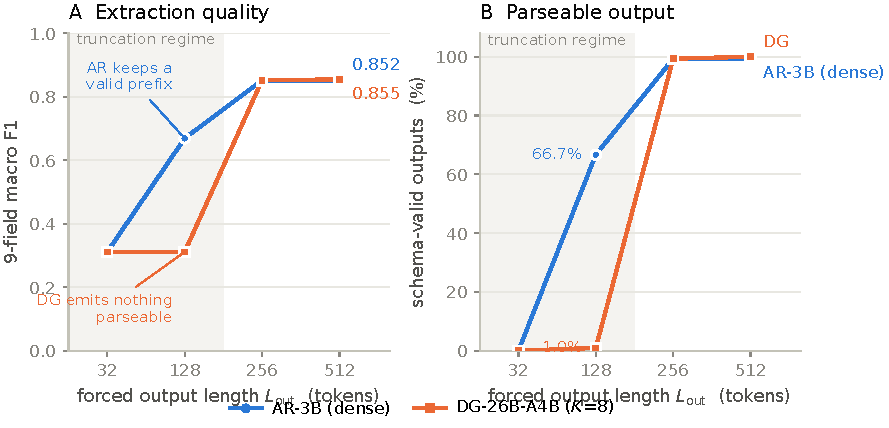
\includegraphics[width=\linewidth]{figures/fig5_quality_vs_length.pdf}
\caption{Quality and parseability against forced output length
(\artifact{results/issue43/}, $n{=}\nPerCell$ per cell, first-object-wins).
The shaded band is the truncation regime, where the output budget is below the
task's natural record length. \textbf{A:} at $L{=}128$ the autoregressive
model retains \arFOneTwentyEight\ F1 while the diffusion model collapses to
\dgFOneTwentyEight. \textbf{B:} the mechanism --- left-to-right decoding
yields a valid \emph{prefix} of fields, while a canvas truncated mid-denoise
yields nothing parseable at all (\arValidTwentyEight\% vs
\dgValidTwentyEight\% schema-valid).}
\label{fig:quality}
\end{figure}

Both models need roughly the task's natural record length before they produce
anything useful, and below it they fail in qualitatively different ways
(Figure~\ref{fig:quality}). This is an autoregressive advantage, and it is the
mirror image of the paper's headline: graceful degradation under a tight
output budget belongs to the architecture that emits tokens in order.

We flag one asymmetry in the figure honestly. The autoregressive curve is flat
from $L{=}256$ to $L{=}512$ at \arThreeBFnine\ only because first-object-wins
discards the rambled continuations; under the old parser it appeared to decay
monotonically, and that apparent decay was defect 3, not a property of the
model. The measured invariance of the diffusion arm across the same range
(\dgNineF\ to $0.8546$) is real and does not depend on parser choice.

\begin{takeaway}
\boxhead{Exchange rate}
At the compute-matched pair, on a decontaminated metric with a fixed parser,
the two architectures are quality-equivalent to within \qualityGap\ F1 at
$L{=}\canvasLength$. Everything that follows compares cost at that quality.
Separately: the \emph{quality-matched} model is not \ARthree\ but \ARoneb,
which reaches \arOneFiveFnine\ --- higher than either. That fact drives
\S\ref{sec:fair}.
\end{takeaway}

\section{The Two Cost Laws}
\label{sec:laws}

With quality fixed, we fit latency as a function of output length for both
architectures on the pinned stack. The two laws have different shapes, and the
rest of the paper is a consequence of that difference.

\subsection{Autoregressive: a line with no floor}

Each output token requires one forward pass over the KV cache, so cost is
linear in output length and independent of how many canvases the output would
have spanned:
\begin{equation}
\label{eq:ar}
T_{\textsc{ar}}(L_{\mathrm{out}}) \;=\; \arBase \;+\; \arSlope \cdot L_{\mathrm{out}}
\qquad\text{(ms)}
\end{equation}
The intercept absorbs prompt prefill (amortised by prefix caching across
requests) and dispatch overhead; the slope is the per-token decode cost. Five
repeats at $L{=}\canvasLength$ give p50 $=$ \arAnchorTwoFive~ms
(CV \arCV\%) and three at $L{=}512$ give \arAnchorFiveOne~ms (CV $0.01\%$);
Eq.~\ref{eq:ar} predicts both within $0.1\%$. The law holds out to $L{=}2048$,
where it predicts \num{12889}~ms against a measured \num{12893}~ms.

\subsection{Block diffusion: a staircase with a high floor}

Diffusion decoding writes onto fixed-size canvases. Within one canvas every
position is denoised in parallel at no additional sequential cost; crossing a
boundary triggers a fresh denoising pass over a new canvas. Cost is therefore
stepwise:
\begin{equation}
\label{eq:dg}
T_{\textsc{dg}}(L_{\mathrm{in}}, L_{\mathrm{out}}) \;=\;
\underbrace{\dgBase}_{\text{base, } K=8} \;+\;
\underbrace{\dgInputSlope \cdot \Delta L_{\mathrm{in}}}_{\text{prefill}} \;+\;
\underbrace{\dgStep \cdot \Bigl(\bigl\lceil \tfrac{L_{\mathrm{out}}}{\canvasLength}\bigr\rceil - 1\Bigr)}_{\text{canvas staircase}}
\qquad\text{(ms)}
\end{equation}
where $\Delta L_{\mathrm{in}}$ is the deviation from the reference prompt of
$\sim$\refPrompt\ tokens. At the reference prompt the prefill term vanishes
and the law reduces to a one-variable staircase.

\paragraph{The edges are exactly where the canvas is}
Figure~\ref{fig:edges}A probes both sides of the first two boundaries.
Growing the output from 240 to \canvasLength\ tokens costs $0.2$\,ms; growing
it from \canvasLength\ to 264 --- eight more tokens, but one more canvas ---
costs $121.7$\,ms. The same pattern repeats at 512.

\begin{figure}[t]
\centering
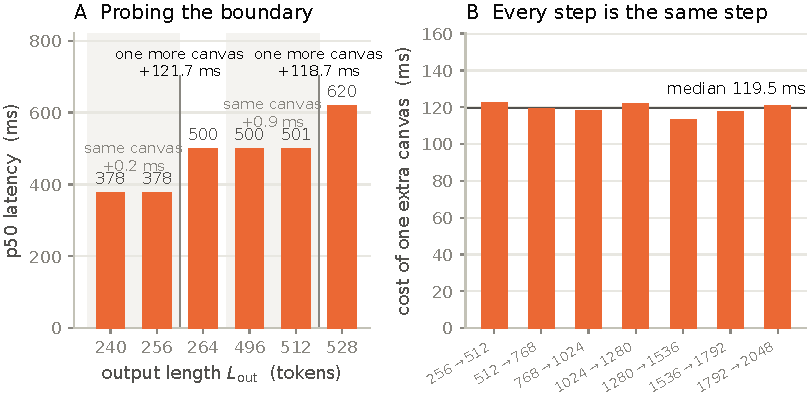
\includegraphics[width=\linewidth]{figures/fig2_canvas_edges.pdf}
\caption{The staircase, probed and then swept
(\artifact{results/issue68\_dg\_L*.json}, $K{=}8$, BGL, $n{=}200$ per point).
\textbf{A:} latency is flat inside a canvas and jumps at the boundary.
\textbf{B:} all seven canvas transitions out to $L{=}2048$ cost the same
within run-to-run noise (range \dgStepLo--\dgStepHi\,ms, median \dgStep\,ms).
An earlier hypothesis that the first extra canvas is cheaper does not
survive: it was a $K{=}32$ versus $K{=}8$ configuration confound.}
\label{fig:edges}
\end{figure}

\paragraph{The steps are uniform}
Figure~\ref{fig:edges}B shows every step out to $L{=}2048$. The spread
(\dgStepLo--\dgStepHi\,ms) is run-to-run noise around a median of
\dgStep\,ms with no systematic trend, so a single global step is an adequate
model over this range. We quote it to one decimal and no further.

\subsection{The second variable: input length}

Equation~\ref{eq:dg} has two variables, and the second one matters more for
diffusion than for autoregression. Sweeping the prompt from roughly 1{,}000 to
6{,}800 tokens (Figure~\ref{fig:input}) gives \arInputSlope\,ms per prompt
token for the autoregressive arm and \dgInputSlope\,ms for the diffusion arm
--- \inputSlopeRatio$\times$ steeper. The mechanism is direct: the
autoregressive model pays for the prompt once and every generated token then
attends to a cached KV, whereas each denoising step re-attends the full
prompt, so prefill is paid $K$ times.

\begin{figure}[t]
\centering
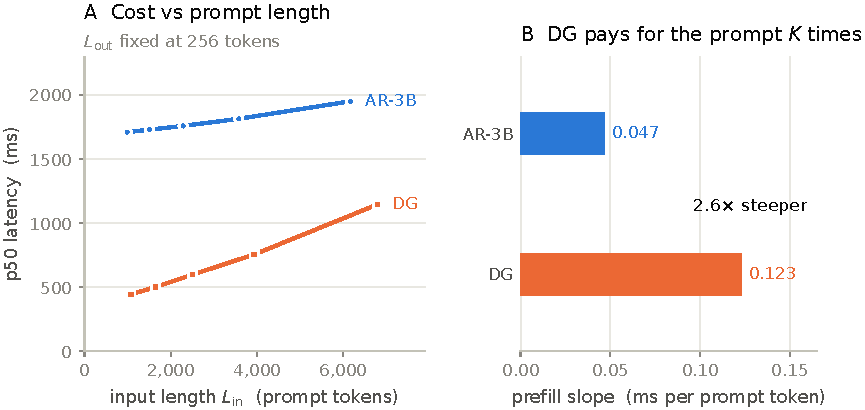
\includegraphics[width=\linewidth]{figures/fig3_input_sweep.pdf}
\caption{Input-length sweep at fixed $L_{\mathrm{out}}{=}\canvasLength$
(\artifact{results/issue44\_\{ar3b,dg\}\_input\_sweep.json}, $n{=}100$ per
point). The prompt is lengthened by repeating the schema block, so the task is
unchanged. \textbf{B} is the finding: the diffusion model's prefill slope is
\inputSlopeRatio$\times$ the autoregressive model's.}
\label{fig:input}
\end{figure}

\begin{caution}
\boxhead{Scope condition, not a footnote}
Every one-variable statement in this paper --- the crossover $L^{*}$, the
per-event ratios, the decision procedure's default mode --- is calibrated at
the reference prompt of $\sim$\refPrompt\ tokens. At longer inputs the
diffusion base rises \inputSlopeRatio$\times$ faster and pushes $L^{*}$ upward.
Extrapolated to a fixed $L_{\mathrm{out}}{=}\canvasLength$, the two curves meet
near $L_{\mathrm{in}} \approx 18{,}000$ tokens, beyond which the
autoregressive model is cheaper at \emph{any} output length. We did not measure
that far; the number is an extrapolation of two fitted slopes and is quoted as
an order of magnitude, not a boundary.
\end{caution}

\subsection{Where the diffusion base actually goes}

The base is not monolithic, and decomposing it changes what the staircase
means. Sweeping the denoising step count $K \in \{2,4,8,16,32,64\}$ at fixed
output length separates a $K$-independent floor from a $K$-dependent denoising
term (Figure~\ref{fig:ksweep}):
\begin{equation}
\label{eq:kfit}
T(K) \;=\; \kfitBase \;+\; \kfitSlope \cdot K
\qquad (R^2 = \kfitRsq)
\end{equation}
The low $R^2$ is itself informative: latency saturates above $K{=}16$, so the
linear term is a poor description at the top of the range and the fit is
carried by the bottom. At the operating point $K{=}8$ the fit puts
\kfitBase\,ms in the $K$-independent floor against \num{20.6}\,ms in the
denoising loop --- \dgPrefillPct\% against \dgDenoisePct\%.

\begin{figure}[t]
\centering
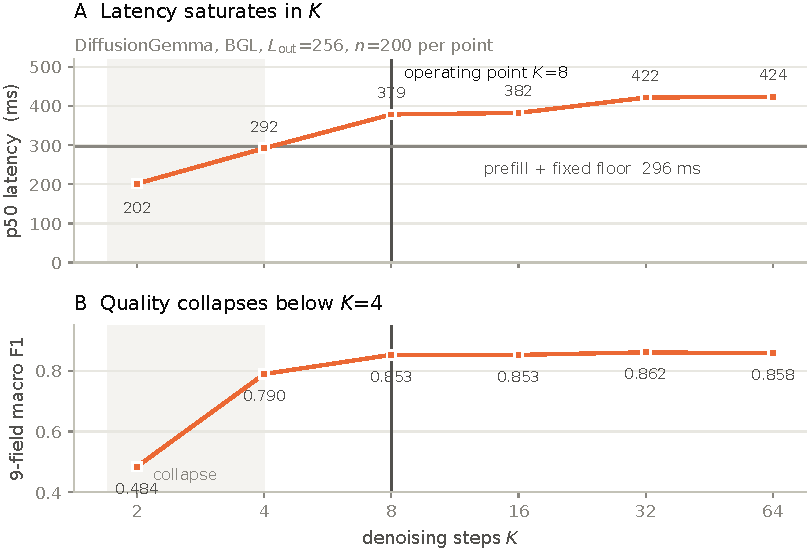
\includegraphics[width=0.92\linewidth]{figures/fig4_ksweep.pdf}
\caption{Denoising-step sweep at $L_{\mathrm{out}}{=}\canvasLength$
(\artifact{results/issue44\_dg\_ksweep\_K*.json}, $n{=}200$ per point).
Latency saturates above $K{=}16$; quality collapses below $K{=}4$ and is flat
above $K{=}8$. Halving $K$ from 8 to 4 saves $\sim$87\,ms because the saving
comes out of the small slice, while F1 falls from \kEightFone\ to \kFourFone\
because the loss comes out of the whole.}
\label{fig:ksweep}
\end{figure}

\begin{keybox}
\boxhead{The shape is structural, not algorithmic}
The denoising loop --- the part that makes this model a diffusion model --- is
\dgDenoisePct\% of its own base cost. The remaining \dgPrefillPct\% is prefill
and fixed dispatch, shared with any prompt-conditioned model. The staircase
therefore comes from the \emph{canvas}, not from the diffusion: any decoder
that emits output in fixed-size blocks would have the same shape, and
diffusion is simply the way this particular model gets block structure. We
name the paper after the block for that reason.
\end{keybox}

\subsection{The crossover}

At the reference prompt and inside the first canvas, the staircase reduces to
its floor and the crossing point is analytic:
\begin{equation}
\label{eq:lcross}
L^{*} \;=\; \frac{\dgBase - \arBase}{\arSlope} \;=\; \crossoverL \ \text{tokens}
\qquad\qquad
\lambda^{*} \;=\; \frac{1000}{\dgBase} \;=\; \crossoverLambda \ \text{events/s}
\end{equation}
Below $L^{*}$ the autoregressive model is cheaper per event; above it the
diffusion model is, until the next canvas edge, where the gap widens again.
$\lambda^{*}$ is the other boundary: with one event in flight, the reciprocal
of the diffusion base is the ceiling on its serial throughput, and above that
rate a queue forms. \S\ref{sec:decision} turns both into a procedure.

\subsection{Both laws survive a change of corpus}

Re-running the sweeps on HDFS leaves both shapes intact. The autoregressive
p50 at $L{=}\canvasLength$ moves from \arBgl\,ms on BGL to \arHdfs\,ms on HDFS
--- $+0.03\%$, well inside the run-to-run CV. The diffusion canvas step moves
from \bglStep\,ms to \hdfsStep\,ms, a $1.7\%$ shift. The prompt content
changes; the shape does not.

\section{The Decision Procedure}
\label{sec:decision}

The two laws produce two crossovers, and the crossovers delimit a region of
the deployment plane. This section turns that derivation into an executable
artifact: a procedure that takes four deployment inputs and returns which
architecture to serve, with the expected cost of the choice. It is
implemented, self-tested, and runnable from a clean checkout with no GPU.

\paragraph{Inputs}
Expected output length $L$ in tokens; arrival rate $\lambda$ in events per
second; whether cross-request batching is available, $B \in \{0,1\}$; and the
Field-F1 a caller will trade for latency, $\tau$. Every constant the procedure
uses traces to a committed artifact; none is hardcoded in the answer.

\paragraph{Guards}
Five guards fire in order and the first that fires wins
(Algorithm~\ref{alg:decide}).

\begin{algorithm}[H]
\caption{Decide which architecture to serve.}
\label{alg:decide}
\begin{algorithmic}[1]
\State $T_{\textsc{ar}} \gets a + bL$;\quad
       $T_{\textsc{dg}} \gets c + s\,(\lceil L/C\rceil - 1)$;\quad
       $r \gets T_{\textsc{ar}}/T_{\textsc{dg}}$
\If{$L < L^{\textsc{dg}}_{\mathrm{nat}}$}
    \Comment{truncation: output below the canvas's natural length}
  \State \Return \textsc{ar}
\ElsIf{$B \wedge \lambda > \lambda^{*}$}
    \Comment{throughput: diffusion serial capacity exhausted}
  \State \Return \textsc{ar}
\ElsIf{$L < L^{*}$}
    \Comment{length: below the latency crossover}
  \State \Return \textsc{ar}
\ElsIf{$\tau < |\Delta F_1|$}
    \Comment{quality: the price exceeds the tolerance}
  \State \Return \textsc{ar}
\Else
  \State \Return \textsc{dg}, with expected per-event speedup $r$
\EndIf
\end{algorithmic}
\end{algorithm}

\noindent
with $a = \arBase$, $b = \arSlope$, $c = \dgBase$, $s = \dgStep$,
$C = \canvasLength$, $L^{*} = \crossoverL$, $\lambda^{*} =
\crossoverLambda$, and $L^{\textsc{dg}}_{\mathrm{nat}} = \naturalLdg$.

\begin{figure}[t]
\centering
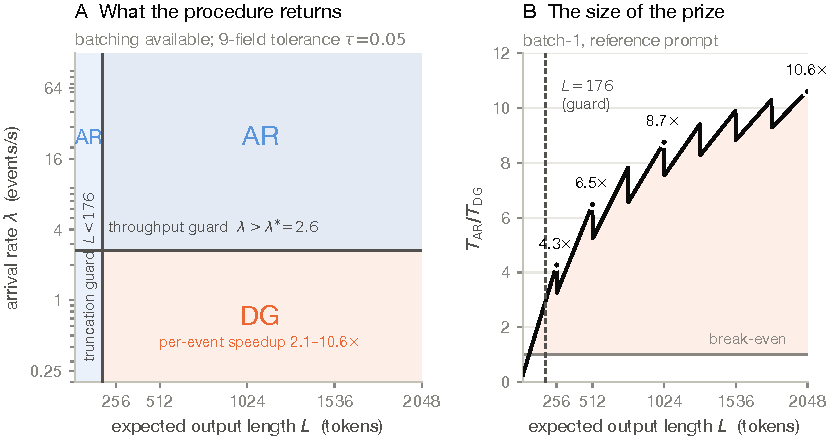
\includegraphics[width=\linewidth]{figures/fig7_decision_map.pdf}
\caption{The procedure drawn as a map. \textbf{A:} the two guards that
actually bind carve the $(L, \lambda)$ plane into three regions. The diffusion
region is bounded below in output length by the truncation guard and above in
arrival rate by the throughput guard. \textbf{B:} inside that region, the
per-event prize --- $T_{\textsc{ar}}/T_{\textsc{dg}}$ --- grows with output
length, dropping back at each canvas edge and climbing again. It reaches
$10.6\times$ at $L{=}2048$.}
\label{fig:decision}
\end{figure}

\paragraph{Two guards subsume the others}
In the current configuration $L^{\textsc{dg}}_{\mathrm{nat}} = \naturalLdg >
L^{*} = \crossoverL$, so any output short enough to sit below the latency
crossover is already below the diffusion model's natural output length and the
truncation guard fires first. Both return \textsc{ar}, so the recommendation
is unchanged; the length guard remains in the procedure because it is the one
that binds as soon as a shorter-canvas variant is configured. The quality
guard is metric-dependent: on the contaminated 12-field metric the price is
$0.039$ and the guard bites, but on the 9-field metric it is $\approx 0$
(\S\ref{sec:exchange}) and the guard is inert. That the guard's behaviour
flips with the choice of metric is exactly why \S\ref{sec:exchange} comes
first.

\paragraph{Worked examples}
Table~\ref{tab:worked} runs six scenarios through the procedure. The ratio
column reports the per-event speedup the diffusion model \emph{would} deliver
even when a non-latency guard selects the autoregressive arm, so the
opportunity cost of each guard is visible rather than hidden.

\begin{table}[h]
\centering
\caption{Six scenarios through the decision procedure. Rows 4--5 carry the
subtlety: the diffusion model would be faster per event, and is still the
wrong choice, because below its natural output length its output is truncated
and stops parsing.}
\label{tab:worked}
\begin{tabular}{@{}lrrccll@{}}
\toprule
\thead{Scenario} & \thead{$L$} & \thead{$\lambda$} & \thead{$B$} & \thead{$\tau$}
  & \thead{Arm} & \thead{$T_{\textsc{ar}}/T_{\textsc{dg}}$ \ \ Guard} \\
\midrule
\tabfont Interactive single-record extraction & \tabfont 176  & \tabfont 0.5 & \tabfont no  & \tabfont 0.05 & \tabfont \textcolor{dgorange}{\bfseries DG} & \tabfont $2.94\times$\quad default \\
\tabfont Long report, batch-1                 & \tabfont 2048 & \tabfont 1.0 & \tabfont no  & \tabfont 0.05 & \tabfont \textcolor{dgorange}{\bfseries DG} & \tabfont $10.6\times$\quad default \\
\tabfont High-volume log pipeline             & \tabfont 256  & \tabfont 64  & \tabfont yes & \tabfont 0.05 & \tabfont \textcolor{arblue}{\bfseries AR} & \tabfont $4.27\times$\quad throughput \\
\tabfont Short field completion               & \tabfont 32   & \tabfont 0.5 & \tabfont no  & \tabfont 0.10 & \tabfont \textcolor{arblue}{\bfseries AR} & \tabfont $0.55\times$\quad truncation \\
\tabfont Tight budget, unknown record size    & \tabfont 128  & \tabfont 0.5 & \tabfont no  & \tabfont 0.05 & \tabfont \textcolor{arblue}{\bfseries AR} & \tabfont $2.14\times$\quad truncation \\
\tabfont Quality-critical, 12-field tolerance & \tabfont 512  & \tabfont 1.0 & \tabfont no  & \tabfont 0.01 & \tabfont \textcolor{arblue}{\bfseries AR} & \tabfont $6.48\times$\quad quality \\
\bottomrule
\end{tabular}
\end{table}

\paragraph{Implementation}
The procedure lives in \artifact{models/decision/procedure.py} with a
command-line interface:
\begin{center}
\ttfamily\small
python -m models.decision -{}-L 512 -{}-lambda 1.0 -{}-no-batching -{}-f1-tolerance 0.05
\end{center}
$T_{\textsc{dg}}$ is injectable: the one-variable law ships as the default and
the two-variable law of Eq.~\ref{eq:dg} swaps in as the only change required,
emitting a warning that its prefill slope applies only near the calibration
prompt. The self-test recomputes $L^{*}$ and $\lambda^{*}$ from the law
constants rather than from stored answers, fires each guard in isolation,
checks all six worked examples, and probes robustness across the measured step
range \dgStepLo--\dgStepHi\,ms: 11 of 11 tests pass.

\begin{caution}
\boxhead{Validity domain}
The constants are calibrated on one \gpuModel\ under vLLM \vllmVersion, BF16,
serial diffusion, for structured extraction over BGL with a
$\sim$\refPrompt-token prompt, at $K{=}8$ and canvas $=\canvasLength$. The
procedure must not be applied to batch-served diffusion, to other canvas
sizes, to materially different input lengths, to other GPUs or runtimes, or
with a tolerance interpreted against the 12-field metric. Outside that box the
shapes should transfer --- they are structural --- but the constants will not.
\end{caution}

\section{The Fair Comparison}
\label{sec:fair}

The decision procedure identifies a region where block-structured decoding
wins on per-event latency. This section asks the sharper question: at a
\emph{fair} comparison point, does the win survive? Fairness has two axes, and
they select different pairs.

\begin{table}[h]
\centering
\caption{Two fair pairs, two different answers. The compute-matched pair is
the right one for per-event claims; the quality-matched pair is the right one
for deployment claims. Confusing them is how a per-event advantage gets
reported as a deployment advantage.}
\label{tab:pairs}
\begin{tabular}{@{}lccc@{}}
\toprule
 & \thead{\ARthree} & \thead{\ARoneb} & \thead{\DG-26B-A4B} \\
\midrule
\tabfont Decoding            & \tabfont dense, autoregressive & \tabfont dense, autoregressive & \tabfont MoE, block diffusion \\
\tabfont Total parameters    & \tabfont 3.0\,B & \tabfont 1.5\,B & \tabfont 26\,B \\
\tabfont Active parameters   & \tabfont 3.0\,B & \tabfont 1.5\,B & \tabfont 4.0\,B (top-8 of 128) \\
\tabfont Weights (bf16)      & \tabfont 6.0\,GB & \tabfont \arOneFiveWeights\,GB & \tabfont \dgWeights\,GB \\
\tabfont 9-field F1 ($L{=}\canvasLength$) & \tabfont \arThreeBFnine & \tabfont \arOneFiveFnine & \tabfont \dgNineF \\
\midrule
\tabfont Matched on          & \multicolumn{1}{c}{\tabfont \emph{compute}} & \multicolumn{1}{c}{\tabfont \emph{quality}} & \tabfont --- \\
\bottomrule
\end{tabular}
\end{table}

\subsection{Where the diffusion model wins}

\paragraph{(a) Per-event latency at batch-1}
Within a canvas the diffusion model emits one token or \canvasLength\ for the
same cost, while the autoregressive model pays per token. The gap therefore
widens with output length: $2.1\times$ at $L{=}128$, $4.3\times$ at
$L{=}\canvasLength$, $6.5\times$ at $L{=}512$, $8.8\times$ at $L{=}1024$, and
$10.6\times$ at $L{=}2048$.

\paragraph{(b) Output-length invariance inside a canvas}
Across $L \in \{32, 64, 128, \canvasLength\}$ the diffusion arm costs
$\approx$379\,ms with a spread under 3\,ms, while the autoregressive arm grows
from 211\,ms to \arAnchorTwoFive\,ms. For a workload whose record size is
variable and not known in advance, this converts a latency distribution into a
latency constant.

\paragraph{(c) Energy}
At the compute-matched pair the diffusion model uses \energyRatio$\times$ less
energy per event, net of idle draw: \dgEnergy\,J against \arThreeEnergy\,J at
forced $L{=}\canvasLength$. The advantage tracks the latency advantage rather
than adding to it --- the two models draw comparable power, and the diffusion
model is simply busy for less time.

\paragraph{(d) A runtime quality knob}
$K$ is a per-request parameter. One deployment serves $K{=}8$ at
\kEightPfifty\,ms and F1 \kEightFone, $K{=}4$ at \kFourPfifty\,ms and
\kFourFone, and $K{=}2$ at \kTwoPfifty\,ms and \kTwoFone, with no model
switch. The autoregressive equivalent is discrete --- deploy a different model
--- so meeting a tightened SLA means routing to a second checkpoint that must
already be resident. Concretely: if a p99 budget tightens to 400\,ms, dropping
$K$ from 8 to 4 meets it at a measured \kFourPninetynine\,ms p99.

\paragraph{(e) Graceful degradation of the right kind}
Under deadline pressure the two architectures fail differently. The diffusion
model degrades in \emph{quality} and always returns a complete canvas; the
autoregressive model degrades in \emph{completeness} and returns a truncated
record. For a caller that validates output against a schema, that difference
is qualitative rather than quantitative: a complete record at F1 \kFourFone\
passes validation, and 46 tokens of a 256-token JSON object does not.

\begin{caution}
\boxhead{The mirror image, stated in the same place}
Property (e) inverts below the natural record length. At $L{=}128$ the
autoregressive model retains \arFOneTwentyEight\ F1 and
\arValidTwentyEight\% schema validity, while the diffusion model falls to
\dgFOneTwentyEight\ and \dgValidTwentyEight\% (\S\ref{sec:exchange},
Figure~\ref{fig:quality}). Diffusion degrades gracefully against a
\emph{time} budget and catastrophically against an \emph{output-length}
budget. Which one an application faces decides which architecture is safer.
\end{caution}

\subsection{Where the autoregressive model wins}

\paragraph{(f) Batched throughput}
Continuous batching converts arrival concurrency into throughput at
\arBatchLo--\arBatchHi$\times$ for the autoregressive arm and
\dgBatchMult$\times$ for diffusion. At $\lambda{=}64$ events/s the effective
per-event cost is $\approx$20\,ms against $\approx$321\,ms --- a $16\times$
advantage under load, running the opposite direction to the batch-1 result.
\S\ref{sec:batching} takes this apart.

\paragraph{(g) Long input}
The diffusion prefill slope is \inputSlopeRatio$\times$ steeper
(\S\ref{sec:laws}), so the advantage narrows as prompts grow and, on the
fitted slopes, closes entirely somewhere around $L_{\mathrm{in}} \approx
18{,}000$ tokens.

\paragraph{(h) Deployment footprint}
This is the one that closes the crossover. The quality-matched autoregressive
model is not \ARthree\ but \ARoneb, which scores \arOneFiveFnine\ on the
9-field metric --- \emph{higher} than the diffusion model --- at
\arOneFiveWeights\,GB against \dgWeights\,GB. Whenever memory or cost matters,
a \footprintRatio$\times$ smaller model that matches quality is the deployment
winner.

\begin{figure}[t]
\centering
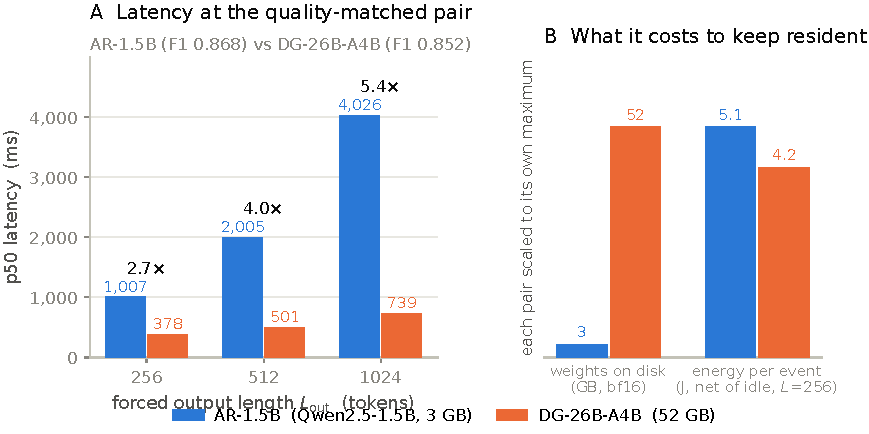
\includegraphics[width=\linewidth]{figures/fig9_deployment.pdf}
\caption{The quality-matched deployment pair. \textbf{A:} at forced output
lengths the diffusion model's advantage is real and grows, because \ARoneb\
rambles well past its natural length ($\sim$\naturalLar\ tokens) and vLLM
still processes every forced token. \textbf{B:} the standing cost of keeping
each model resident. Energy per event is net of idle draw; the two energy runs
recorded different idle baselines (52.6\,W and 58.6\,W), so treat the energy
comparison as indicative rather than as a tight measurement.}
\label{fig:deploy}
\end{figure}

\subsection{So where does that leave the diffusion model?}

At \emph{natural} output length the contest is close: \ARoneb\ completes a
record in 665.7\,ms p50 at 138 output tokens on the pinned stack, against the
diffusion model's \dgTwoFive\,ms. A $1.8\times$ gap, on a model that is
\footprintRatio$\times$ larger, is not a deployment argument.

At \emph{forced} output length the picture changes, and this is the surviving
niche. When an application requires $L \geq 512$ tokens of structured output
--- a multi-field incident report, a full trajectory plan, a long structured
summary --- \ARoneb's latency quadruples to \arOneFiveFiveOne\,ms while the
diffusion model's grows by 32\% to \dgFiveOne\,ms
(Figure~\ref{fig:deploy}A). At $L{=}1024$ the gap is $5.4\times$.

\begin{keybox}
\boxhead{When block diffusion is the right choice}
All five conditions must hold together:
\begin{enumerate}[nosep]
  \item Output length $\geq 512$ tokens, and \emph{forced} --- the application
    needs a full structured record, not the shortest one the model would emit.
  \item Batch-1 by \emph{requirement}, not by low load: tenant isolation,
    interactivity, or a human-initiated cold path. If batching is available,
    \S\ref{sec:batching} settles it.
  \item Completeness is validated. The caller checks the output against a
    schema and cannot use a prefix.
  \item The quality floor exceeds what \ARoneb\ delivers. If it does not, the
    \arOneFiveWeights\,GB model wins on every axis that is not per-event
    latency.
  \item A \dgWeights\,GB resident footprint is acceptable --- data centre, not
    edge.
\end{enumerate}
\vspace{2pt}
That is a narrow niche. It is also a real one, and it is not primarily about
speed: it is the combination of per-event speed, a per-request quality knob,
and a guarantee of complete output under deadline pressure.
\end{keybox}

\subsection{One autoregressive advantage we did not expect}

The autoregressive arm's latency distribution is dramatically tighter. Across
the 300 individual events of one anchor run at $L{=}\canvasLength$, its
per-event coefficient of variation is \arEventCV\% and its maximum-to-median
ratio is \arMaxMed$\times$; the diffusion arm's CV is \dgEventCV\% with a
max/median of \dgMaxMed$\times$, driven by mixture-of-experts routing
variability and warm-up on the first events of a run. (These are
\emph{within}-run figures, distinct from the run-to-run p50 CVs of \arCV\%
and \dgCV\% quoted in \S\ref{sec:intro}.) For capacity
planning this favours the autoregressive model directly: a tighter
distribution means less provisioned headroom. Both models are deterministic at
temperature 0 --- across five repeats of 300 events, outputs were identical
--- so determinism is not a differentiator between them.

\section{The Batching Boundary}
\label{sec:batching}

The per-event crossover favours the diffusion model in a narrow region, but a
deployment serves an arrival stream, not one event. Under batching the picture
does not merely shift --- it inverts, by roughly two orders of magnitude
(Figure~\ref{fig:batching}).

\begin{figure}[t]
\centering
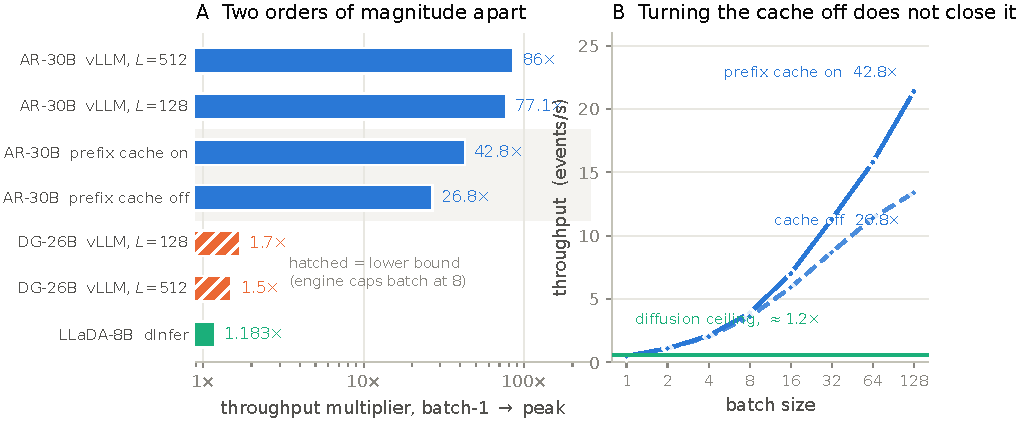
\includegraphics[width=\linewidth]{figures/fig6_batching.pdf}
\caption{\textbf{A:} batch-1 to peak throughput multipliers. The split runs
along architecture, not runtime: two diffusion models on two different engines
sit at $\approx$1--$1.7\times$, while the autoregressive model on vLLM ranges
from \cacheOffMult$\times$ to \arBatchHi$\times$ depending on output length
and cache configuration. The DiffusionGemma bars are lower bounds --- the
engine caps its batch at 8 (\S\ref{sec:setup}) --- which is why the LLaDA
measurement on dInfer is the load-bearing one. \textbf{B:} the direct test.
Disabling prefix-cache reuse costs the autoregressive model $37\%$ of its
headroom and leaves \cacheOffMult$\times$ standing, more than twenty times the
diffusion ceiling.}
\label{fig:batching}
\end{figure}

\subsection{The gap, and a second runtime}

On vLLM the autoregressive model sustains \arBatchLo$\times$ at $L{=}128$ and
\arBatchHi$\times$ at $L{=}512$. DiffusionGemma on the same engine sustains
\dgBatchVllmHi$\times$ and \dgBatchVllmLo$\times$ --- but those numbers were
measured with the batch capped at 8 by the mixed-phase crash, so they are
lower bounds on what vLLM could do, not measurements of a ceiling.

The control that makes the result more than a bug report is LLaDA-8B on
dInfer: a different model family (dense rather than mixture-of-experts), a
different runtime, and a diffusion-native one. It sustains
\dgBatchMult$\times$, flat from batch 2 to batch 64. Two runtimes, two model
families, the same ceiling.

\subsection{We tested the mechanism, and it is not the whole story}

The standing explanation for the ceiling is that bidirectional attention
invalidates the KV-cache reuse that makes autoregressive batching cheap,
leaving the diffusion model compute-bound at batch-1 with no bandwidth-bound
headroom for batching to convert. That explanation is plausible, and it is
testable in one direction: if KV-cache reuse is what creates the headroom,
removing it should remove the headroom.

It does not. Re-running the autoregressive batch sweep with prefix caching
disabled drops the multiplier from \cacheOnMult$\times$ to
\cacheOffMult$\times$ --- a real effect, and clearly the cache is doing work
--- but \cacheOffMult$\times$ is still more than twenty times the diffusion
ceiling of \dgBatchMult$\times$. Cache reuse therefore accounts for part of
the gap and cannot account for the rest.

\begin{caution}
\boxhead{Correlation, and how much of the mechanism we actually isolated}
The $\approx$1$\times$ diffusion ceiling is measured and reproduces across two
runtimes and two model families. The \emph{cause} is not isolated. The KV-cache
hypothesis is now partly falsified as a complete explanation. Remaining
candidates: mixture-of-experts routing that varies across denoising steps and
invalidates cached activations; sheer model size, since the diffusion model is
\footprintRatio$\times$ larger than the quality-matched autoregressive model
and memory pressure binds earlier; and kernel maturity, since vLLM's
autoregressive path is years more optimised than its diffusion path. We
disentangle none of these. The ceiling is real; the explanation is open.
\end{caution}

\subsection{Tuning the canvas does not move the crossover}

DiffusionGemma's canvas length is a configuration parameter, so we swept it.
At canvas $=128$ the base falls to \canvasOneTwentyEightBase\,ms
($-2.4\%$) and 9-field F1 rises to \canvasOneTwentyEightFone\ --- a free
improvement on both axes. At canvas $=64$ the base rises $48\%$, because the
per-canvas fixed overhead is now paid twice as often; that setting is not
viable.

Neither setting moves the per-event crossover. $L^{*}$ is set by the prefill
cost that dominates the base --- \dgPrefillPct\% of it at $K{=}8$
(\S\ref{sec:laws}) --- and prefill does not shrink when the canvas does.
Tuning the canvas trades quality against step count. It does not buy a
different crossover.

\section{Negative Results}
\label{sec:negative}

We set out to find regimes where the diffusion model beats the autoregressive
baseline, and generated hypotheses accordingly. Six were refuted and three
earlier claims were withdrawn. They are reported here at the same length and
in the same register as the confirmations, because a paper whose central
methodological claim is ``price the baseline before you compare against it''
has exactly one asset, and that asset is spent the moment a negative result
gets softened into a footnote.

\subsection{Six refuted hypotheses}

\begin{table}[h]
\centering
\caption{Six hypotheses of ours that did not survive measurement.}
\label{tab:refuted}
\begin{tabularx}{\linewidth}{@{}p{4.6cm}L@{}}
\toprule
\thead{Hypothesis} & \thead{What we measured instead} \\
\midrule
\tabfont Joint denoising resists input perturbation
  & \tabfont The diffusion model degraded more in \textbf{10 of 10} categories, by up to $8.2\times$ the autoregressive drop. Discussed below. \\
\tabfont Bidirectional conditioning wins at infilling
  & \tabfont \ARthree\ scores $0.993$--$0.999$ across all suffix sizes; the diffusion model holds to $0.960$ then falls to $0.753$ at $S{=}8$. Discussed below. \\
\tabfont Diffusion has a refinement mechanism that pays off
  & \tabfont It has the mechanism --- selective re-masking gains $+0.023$ F1 over three rounds --- but after three rounds it still trails the autoregressive model after one. The mechanism is real; the win is not. \\
\tabfont Diffusion beats autoregression under bounded deadlines
  & \tabfont This was defect 4. The autoregressive model does complete within the deadline; the metric had been counting valid falsy values as missing keys (\S\ref{sec:setup}). \\
\tabfont Wide-schema cost scales as $O(F^2)$ for diffusion
  & \tabfont Never measured. The consistency metric is three hardcoded rules over four fields at \emph{every} schema width, so the curve it produces cannot show quadratic structure in $F$. The framing is dropped, not softened. \\
\tabfont Quality is invariant to output length
  & \tabfont Quality rises steeply with $L$ and then plateaus (\S\ref{sec:exchange}). The apparent invariance came from the contaminated 12-field metric. \\
\bottomrule
\end{tabularx}
\end{table}

\paragraph{Perturbation robustness, refuted in every category}
We predicted that denoising a whole canvas jointly would make the diffusion
model more tolerant of noisy input than left-to-right decoding. Across ten
perturbation categories at full intensity, it was worse in all ten. Two
categories --- whitespace and abbreviation --- left the autoregressive model
completely flat while costing the diffusion model $0.081$ and $0.005$ F1. The
largest ratio is separator changes, at $8.2\times$. One hypothesis for the
direction: left-to-right conditioning propagates input noise forward only,
while bidirectional conditioning also propagates it backward. We did not test
that, and it stays a hypothesis.

\paragraph{Infilling, refuted for a reason worth stating}
The prediction was structural rather than statistical: with a fixed right
context, suffix tokens are never in the denoised set, so the diffusion model
should preserve them byte-identically by construction, while an autoregressive
model must regenerate them. The experiment ($S \in \{0,2,4,8\}$ suffix fields,
$n{=}50$) refuted it, but the mechanism matters --- the autoregressive model
scores $0.993$--$0.999$ because it trivially regenerates the whole record from
the prompt. This task is copy-heavy, and copying is something autoregressive
decoding does well. The structural argument may still hold where the suffix is
long and cannot be regenerated from context, such as code infilling. It does
not hold on short JSON fields, which is what we measured, so it is not a claim
we make.

\subsection{Three withdrawn claims}

\begin{table}[h]
\centering
\caption{Three claims that appeared in earlier drafts and are cut from this
one. Withdrawn claims are removed, not qualified.}
\label{tab:withdrawn}
\begin{tabularx}{\linewidth}{@{}p{4.6cm}L@{}}
\toprule
\thead{Claim} & \thead{Why it is gone} \\
\midrule
\tabfont A classical parser matches LLM extraction
  & \tabfont Field-F1 $0.68$ against $0.85$; the gap is too large. Worse, our ``Drain''~\cite{drain} was a regex fallback rather than the reference implementation, and the fallback and the gold generator are the same code, so on semantic fields it was grading itself. \\
\tabfont Structural and semantic fields separate cleanly
  & \tabfont The semantic gold labels are placeholder output of that same parser, and one of them is a constant. ``Semantic F1'' may be measuring agreement with a regex. \\
\tabfont An M/D/1 queue predicts diffusion latency under load
  & \tabfont It matches the measured saturation knee under Poisson arrivals and stops being predictive under bursty (MMPP) arrivals, which is what log streams actually look like. \\
\bottomrule
\end{tabularx}
\end{table}

\begin{takeaway}
\boxhead{A pattern in the refutations}
Every refuted hypothesis had, at some earlier point, appeared to be confirmed.
In each case the apparent confirmation traced to an artifact of our own
harness rather than to a property of either architecture: the bounded-deadline
result was the completeness metric, the length-invariance result was the
contaminated metric, and the perturbation and refinement arms ran a
mis-provenanced model. The measurement discipline of \S\ref{sec:setup} is not
a preamble to the results. It is what separates these six from the ones we
kept.
\end{takeaway}

\section{Threats to Validity}
\label{sec:threats}

\paragraph{The two arms are not size-matched}
This is the largest threat and the reason \S\ref{sec:fair} exists. The
compute-matched pair matches active parameters (3.0\,B against 4.0\,B), not
model size: DiffusionGemma carries 26\,B total parameters and \dgWeights\,GB
of weights against \ARthree's 6.0\,GB. Every per-event latency claim in this
paper is made at that pair, and every per-event claim therefore favours the
diffusion model by an amount we cannot fully price. The deployment comparison
against \ARoneb\ is our attempt to bound it, not to eliminate it.

\paragraph{One GPU}
All measurements are on a single \gpuModel. The cost \emph{shapes} --- a line
against a staircase --- are structural and should transfer. The fitted
constants ($\arBase$, $\arSlope$, $\dgBase$, $\dgStep$) are A100-specific, and
so, therefore, are $L^{*}$ and $\lambda^{*}$. We have no H100 comparison.

\paragraph{One model family carries the staircase}
The staircase is established on DiffusionGemma-26B-A4B and confirmed across
two corpora (BGL step \bglStep\,ms; HDFS \hdfsStep\,ms). The LLaDA-8B arm
under dInfer was measured and is \emph{inconclusive}: dInfer's prefix and
vicinity KV-cache paths error on prompts of 632 tokens or more, forcing a
cache-less mode that inflates absolute latency by roughly $30\times$ and
introduces variance that swamps any block-length stepping. We therefore cannot
say the staircase reproduces on a second diffusion family --- only that its
form should hold for any canvas-bound decoder, and that confirming it needs a
production-grade diffusion runtime with a working cache, which did not exist
at the time of writing.

\paragraph{The batching cap is measured; its cause is not}
\S\ref{sec:batching} reports a direct test that falsifies KV-cache reuse as a
\emph{complete} explanation and leaves three candidate causes untested.
Separately, the dInfer control that licenses calling the ceiling
architectural was itself run cache-less because of the bug above --- so a
cache-based mechanism is being argued partly from a cache-less measurement.
We state the ceiling as a reproduced correlation.

\paragraph{The one-variable law is a projection}
The cost law is two-variable (Eq.~\ref{eq:dg}). $L^{*} = \crossoverL$ is its
projection at a \refPrompt-token prompt. At longer inputs the steeper
diffusion prefill slope raises the base and pushes $L^{*}$ upward, and the
one-variable form under-predicts badly: on an accidental input-length sweep
(a schema-widening experiment that lengthens the prompt) it under-predicted by
$+58\%$ and $+112\%$ at the two largest widths, where the autoregressive law
reproduced the same cells to within $0.4\%$. The crossover is valid near its
calibration prompt and nowhere else.

\paragraph{$K$ is pinned at 8}
Every number assumes $K{=}8$ unless stated. The base is $K$-dependent: at
$K{=}32$ it was \dgOldBase\,ms, which moves $L^{*}$ from \crossoverL\ to $65$
and $\lambda^{*}$ from \crossoverLambda\ to $2.4$. An earlier finding that
``the first extra canvas is 16\% cheaper'' dissolved once this confound was
identified --- it was a $K{=}32$ measurement compared against $K{=}8$ ones.
The decision procedure takes the base as an input so the crossovers recompute.

\paragraph{Long-context memory is unmeasured}
We attempted to measure \ARoneb's GPU memory at context lengths to 32k with
\texttt{enforce\_eager}, and \texttt{torch.cuda.max\_memory\_allocated}
returned zero because vLLM manages its own pool. The latency side confirms
autoregressive input sensitivity (43.8\,ms at 1k context rising to 435.9\,ms
at 16k), but the memory question is open. The absence of a growing KV cache
may give the diffusion model a flatter memory curve at long context. We did
not measure it and do not claim it.

\paragraph{Energy is measured against two different idle baselines}
The compute-matched energy comparison (\arThreeEnergy\,J against
\dgEnergy\,J) was taken in one session at 52.6\,W idle. The \ARoneb\ figure
(\arOneFiveEnergy\,J) comes from a later session at 58.6\,W idle. Net-of-idle
subtraction makes them roughly comparable but not tightly so, and the
quality-matched energy comparison in \S\ref{sec:fair} should be read as
indicative.

\paragraph{Cold-start cost is not reported}
Earlier drafts of this work quoted a cold-start comparison. The measured
values in our artifacts are engine-initialisation times dominated by runtime
setup rather than by weight loading, and they do not support the comparison
that was drawn from them. The row is removed rather than re-derived.

\paragraph{No confidence intervals outside the anchors}
Five repeats exist at the two anchor cells, which is where the CV figures come
from. Most other cells are single runs of $n{=}\nPerCell$ events. We report
run-to-run spread where we measured it and do not manufacture error bars where
we did not.

\section{Conclusion}
\label{sec:conclusion}

Autoregressive and block-diffusion decoders do not sit at two points on a
latency scale. They have different cost \emph{shapes}: a line with no floor,
and a staircase with a floor that is \dgPrefillPct\% prefill. Almost
everything a deployment needs to know follows from that difference and from
where the two shapes cross.

We measured both laws on one pinned stack, showed the staircase has sharp
edges exactly at canvas boundaries and uniform steps out to $L{=}2048$, found
the second variable that makes the diffusion law two-dimensional, and turned
the pair into a decision procedure whose constants all trace to committed
artifacts. Then we asked the question that motivated the work: does the
per-event advantage survive a fair comparison? At short output it does not.
The quality-matched autoregressive model is \footprintRatio$\times$ smaller,
batches \arBatchMult$\times$ better, and pays \inputSlopeRatio$\times$ less
per prompt token. At forced long output under a batch-1 constraint it does
survive, by $4.0$--$5.4\times$, and it brings two structural properties the
autoregressive model has no equivalent for: a per-request quality knob, and a
complete record at every point on the quality curve.

Two things we would emphasise to anyone extending this. First, the shape is
caused by the \emph{block}, not by the diffusion --- the denoising loop is
\dgDenoisePct\% of the base cost, so any decoder emitting fixed-size blocks
would inherit the same staircase, and the interesting design space is block
size rather than denoising schedule. Second, the four defects that biased our
own harness against the autoregressive baseline all lived in the
infrastructure around the model rather than in the model itself. That is not a
coincidence; it is what a comparison harness does when the person writing it
would prefer one of the two answers. The five checks in
\artifact{CHECKLIST.md} each take under five minutes, and each of them caught
something that had already changed a headline number.


\bibliographystyle{plain}
\bibliography{references}

\end{document}
